\section{Thiết kế cơ sở dữ liệu}
\label{sec:3-4-database}


Dựa theo những yêu cầu và thiết kế, cơ sở dữ liệu của hệ thống VieVu được thiết kế theo mô hình quan hệ như minh họa trong Hình~\ref{fig:3-4-database}. % <<< !!! NHỚ THAY LABEL FIG ĐÚNG !!!
Hệ thống sử dụng CSDL PostgreSQL được host và quản lý trên nền tảng Supabase. Các bảng dữ liệu chính bao gồm
\subsection{Các bảng dữ liệu chính}
\begin{itemize}
    \item \textbf{trips}: Bảng trung tâm lưu trữ thông tin về các chuyến đi. Các trường chính gồm \texttt{id} (PK), \texttt{owner\_id} (FK đến \texttt{profiles}), \texttt{name}, \texttt{description}, \texttt{start\_date}, \texttt{end\_date}, \texttt{status}, \texttt{is\_published}, \texttt{cover} (URL ảnh bìa), \texttt{locations} (mảng xâu kí tự tên các địa điểm chính của chuyến đi).

    \item \textbf{trip\_participants}: Bảng liên kết nhiều-nhiều giữa người dùng (\texttt{profiles}) và chuyến đi (\texttt{trips}), thể hiện thành viên tham gia và vai trò của họ trong chuyến đi. Chứa \texttt{user\_id}, \texttt{trip\_id}, \texttt{role} ('owner', 'member',v.v.), \texttt{is\_banned}.

    \item \textbf{saved\_services}: Lưu trữ các dịch vụ/địa điểm được người dùng lưu lại để cân nhắc lên lịch trình cho chuyến đi. Chứa \texttt{id} (PK), \texttt{trip\_id} (FK đến \texttt{trips}), \texttt{external\_link}, \texttt{name}, \texttt{location\_name}, \texttt{latitude}, \texttt{longitude}, \texttt{price}, \texttt{event\_date},v.v.

    \item \textbf{trip\_itineraries}: Lưu trữ lịch trình chi tiết theo ngày/giờ của chuyến đi, liên kết với các dịch vụ đã lưu. Gồm \texttt{id} (PK), \texttt{trip\_id} (FK đến \texttt{trips}), \texttt{service\_id} (FK đến \texttt{saved\_services}), \texttt{title}, \texttt{latitude}, \texttt{longitude}, \texttt{ts\_time} (thời gian bắt đầu).

    \item \textbf{trip\_reviews}: Lưu trữ đánh giá của thành viên về chuyến đi. Chứa \texttt{id} (PK), \texttt{trip\_participant\_id} (FK đến \texttt{trip\_participants}), \texttt{review}, \texttt{rating}, \texttt{trip\_id}, \texttt{is\_edited}.
    
    \item \textbf{user\_ratings}: Lưu trữ đánh giá giữa các thành viên trong chuyến đi. Chứa \texttt{id} (PK), \texttt{rater\_id} (FK đến \texttt{profiles}), \texttt{rated\_id} (FK đến \texttt{profiles}), \texttt{trip\_id}, \texttt{rating}, \texttt{comment}.

    \item \textbf{locations}: Lưu trữ dữ liệu về các điểm đến ở Việt Nam (các tỉnh thành, quận,v.v.). Chứa \texttt{id} (PK), \texttt{name}, \texttt{cover} (URL ảnh), \texttt{latitude}, \texttt{longitude}, \texttt{parent\_id} (nếu là địa điểm con).

    \item \textbf{attractions}: Lưu trữ thông tin chi tiết về các điểm tham quan du lịch cụ thể. Chứa \texttt{id} (PK), \texttt{location\_id} (FK đến \texttt{locations}), \texttt{name}, \texttt{images} (array URL), \texttt{address}, \texttt{latitude}, \texttt{longitude}, \texttt{phone}, \texttt{avg\_rating}, \texttt{rating\_count},v.v.

    % \item \textbf{attraction\_types}: Phân loại các điểm tham quan thuộc vào loại hình du lịch nào. Chứa \texttt{id} (PK), \texttt{attraction\_id} (FK đến \texttt{attractions}), \texttt{travel\_type\_id} (FK đến \texttt{travel\_types}), \texttt{type\_name}.

    \item \textbf{travel\_types}: Bảng danh mục các loại hình du lịch (ví dụ: 'Núi', 'Bãi Biển', 'Công viên'). Chứa \texttt{id} (PK), \texttt{name}, \texttt{parent\_id} (nếu có phân cấp).

    \item \textbf{chats}: Đại diện cho một cuộc hội thoại, có thể là nhóm hội thoại của một chuyến đi hoặc nhắn tin riêng giữa các người dùng. Chứa \texttt{id} (PK), \texttt{name} (tên cuộc hội thoại, nếu là nhóm), \texttt{avatar} (URL ảnh đại diện, nếu là nhóm), \texttt{trip\_id} (FK đến \texttt{trips}, nếu là chat của chuyến đi, có ràng buộc UNIQUE).
    
    \item \textbf{chat\_summaries}: Quản lý thông tin tóm tắt về các cuộc hội thoại. Chứa \texttt{id} (PK), \texttt{updated\_at}, \texttt{last\_message\_id}, \texttt{chat\_id} (Fk đến bảng chat), \texttt{summary}, \texttt{is\_converted} (đã được cập nhật vào lịch trình hay chưa), \texttt{readings} (dạng markdown để người dùng dễ đọc).

    \item \textbf{chat\_members}: Lưu thành viên của cuộc hội thoại. Chứa \texttt{id} (PK), \texttt{user\_id}, \texttt{chat\_id}, \texttt{last\_seen\_message\_id}.

    \item \textbf{messages}: Lưu trữ nội dung tin nhắn và các trạng thái của tin nhắn. Gồm \texttt{id} (PK), \texttt{chat\_id} (FK đến \texttt{chat}), \texttt{content}, \texttt{chat\_member\_id} (FK đến \texttt{chat\_members}), \texttt{is\_travel\_related} (đánh dấu có nên được tổng hơp hay không).

    % \item \textbf{message\_reactions}: Lưu trữ phản hồi (reaction) cho tin nhắn. Gồm \texttt{id} (PK), \texttt{message\_id} (FK đến \texttt{messages}), \texttt{reactor\_id} (FK đến \texttt{profiles}), \texttt{chat\_id}, \texttt{chat\_member\_id}, \texttt{emotion}.

    \item \textbf{notifications}: Lưu trữ thông báo gửi đến người dùng và là lời mời tham gia chuyến đi. Gồm \texttt{id} (PK), \texttt{receiver\_id} (FK đến \texttt{profiles}), \texttt{sender\_id} (FK đến \texttt{profiles}), \texttt{type}, \texttt{content}.

    \item \textbf{user\_preferences}: Lưu trữ sở thích du lịch của người dùng từ khảo sát ban đầu và cách hành vi người dùng trong app. Gồm \texttt{id} (PK), \texttt{user\_id} (FK đến \texttt{profiles}), \texttt{budget}, \texttt{prefs\_df} (ma trận sở thích người dùng), \texttt{avg\_rating}, \texttt{rating\_count}.

    \item \textbf{preference\_history}: Có thể lưu lịch sử thay đổi sở thích hoặc điểm số sở thích thông qua hành vi sử dụng. Gồm \texttt{id} (PK), \texttt{user\_id} (FK đến \texttt{profiles}), \texttt{travel\_type}, \texttt{previous\_score}, \texttt{new\_score}, \texttt{action}.

    % \item \textbf{search\_history}: Lưu lịch sử tìm kiếm của người dùng. Gồm \texttt{id} (PK), \texttt{user\_id} (FK đến \texttt{profiles}), \texttt{keyword}.

   
\end{itemize}
\noindent
Thiết kế các bảng dữ liệu này phù hợp cho việc lưu trữ thông tin cốt lõi, hỗ trợ các chức năng chính của ứng dụng VieVu như quản lý chuyến đi, lập lịch trình, tương tác xã hội và gợi ý du lịch. Mối quan hệ giữa các bảng đảm bảo tính toàn vẹn dữ liệu và cho phép truy vấn thông tin phức tạp để phục vụ các yêu cầu nghiệp vụ của hệ thống.


\subsection{Tích hợp với các bảng hệ thống của Supabase}


Bên cạnh các bảng dữ liệu được định nghĩa riêng cho ứng dụng trong schema `public`, hệ thống VieVu còn tích hợp và tận dụng các dịch vụ cốt lõi do Supabase cung cấp, chủ yếu thông qua hai bảng hệ thống sau:
\begin{itemize}
    \item \textbf{auth.users (Supabase Auth):} Bảng tích hợp sẵn của Supabase quản lý thông tin xác thực và định danh người dùng cơ bản. Bảng \texttt{profiles} của VieVu liên kết trực tiếp với bảng này qua \texttt{id} (UUID) để mở rộng thông tin hồ sơ.

    \item \textbf{storage.objects (Supabase Storage):} Hệ thống lưu trữ tệp của Supabase, được VieVu sử dụng để lưu các đối tượng media như ảnh đại diện, ảnh bìa, ảnh địa điểm. Các bảng ứng dụng liên quan sẽ lưu đường dẫn hoặc ID tham chiếu đến các đối tượng trong Storage này.

    % \item \textbf{pg\_cron (Scheduled Tasks):} Hệ thống tận dụng extension \texttt{pg\_cron} của PostgreSQL (được hỗ trợ bởi Supabase) để lên lịch và thực thi các tác vụ nền định kỳ một cách tự động, ví dụ như cập nhật trạng thái chuyến đi hoặc gửi thông báo tổng hợp.

    % \item \textbf{Row Level Security (RLS):} Các chính sách Bảo mật Cấp độ Hàng (RLS) được định nghĩa và áp dụng trên các bảng dữ liệu quan trọng để kiểm soát chi tiết quyền truy cập (CRUD) của người dùng đối với từng dòng dữ liệu cụ thể, tăng cường an toàn và bảo mật.
\end{itemize}
Việc tích hợp này cho phép hệ thống VieVu tận dụng cơ sở hạ tầng mạnh mẽ của Supabase cho các tác vụ nền tảng như xác thực người dùng và lưu trữ tệp tin, giúp tập trung hơn vào việc xây dựng các tính năng nghiệp vụ đặc thù của ứng dụng.

\subsection{Triggers, Functions và Cronjob}

Ngoài các bảng dữ liệu chính, hệ thống còn sử dụng 3 tính năng của cơ sở dữ liệu PostgreSQL là triggers, functions và cronjob để tự động hóa một số quy trình trong cơ sở dữ liệu. Cụ thể:
\begin{itemize}
    \item \textbf{udpate\_trip\_status\_job}: Một tác vụ chạy nền định kỳ trong \texttt{pg\_cron} giúp kiểm tra và cập nhật trạng thái chuyến đi đúng với giờ xuất phát và kết thúc.
    
    \item \textbf{search\_history\_limit}: Trigger giới hạn lịch sử tìm kiếm của người dùng (tối đa 10). Tự động xóa lịch sử cũ nhất khi có lịch sử mới được thêm vào.
    \item \textbf{fetch\_nearby\_places}: Function tìm kiếm điểm tham quan (\texttt{attractions}) lân cận dựa trên khoảng cách địa lý và bán kính. Tự động trả về các địa điểm gần nhất nếu không đủ kết quả trong bán kính yêu cầu.
    % --- Hết mục mới ---
    \item \textbf{get\_attractions}: Function truy vấn điểm tham quan (\texttt{attractions}) với các tùy chọn lọc linh hoạt (theo ID địa điểm lớn, lân cận, loại hình du lịch) và sắp xếp (theo \texttt{hot\_score} hoặc điểm đánh giá). Trả về kết quả kèm thông tin loại hình (JSON) và điểm đánh giá cân bằng.
    
    % --- search_profiles_and_trips rút gọn ---
    \item \textbf{search\_profiles\_and\_trips}: Function tìm kiếm toàn văn (FTS) trên \texttt{profiles} (tên người dùng) và \texttt{trips} (tên chuyến đi, địa điểm) theo từ khóa. Kết quả được kết hợp, xếp hạng theo độ liên quan (ưu tiên tên chuyến đi), hỗ trợ lọc theo loại và phân trang.
\end{itemize}

\begin{figure}[H]
    \centering  
    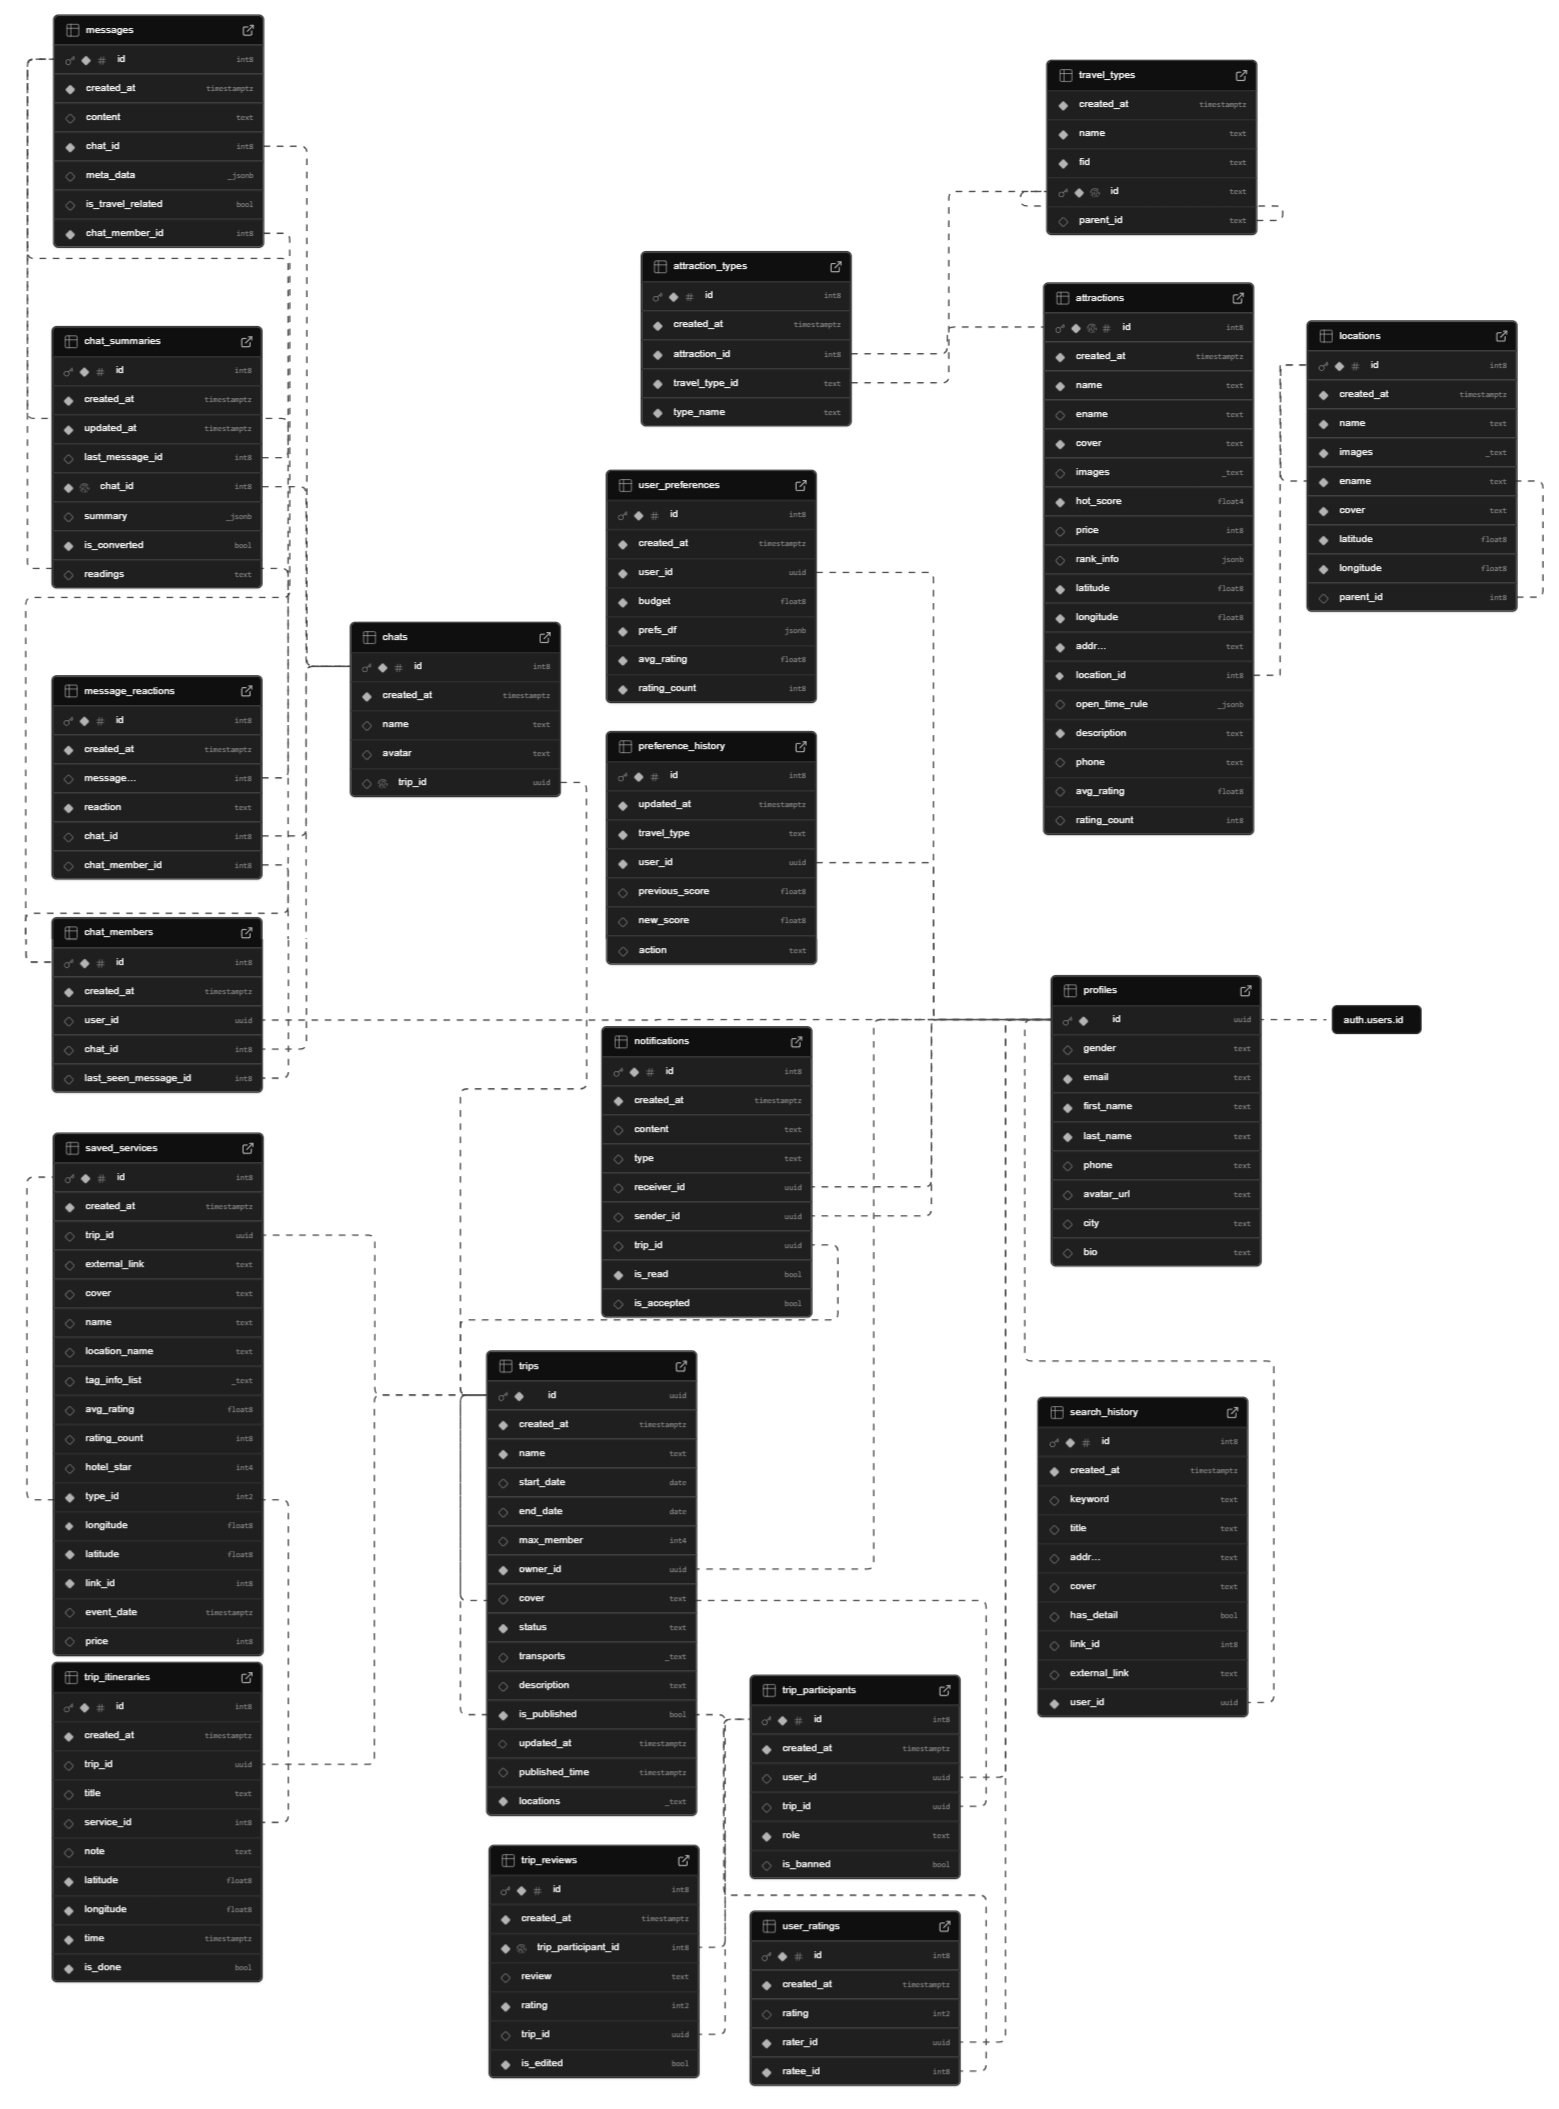
\includegraphics[width=1.1\textwidth]{figures/c3/test2.png}
    \caption{Cấu trúc cơ sở dữ liệu.}
    \label{fig:3-4-database}
\end{figure}

